\documentclass[11pt]{article}
\usepackage[margin=1in]{geometry}
\usepackage{amsmath,amssymb,amsthm}
\usepackage{booktabs}
\usepackage{graphicx}
\usepackage{microtype}
\usepackage[htt]{hyphenat}
\emergencystretch=3em
\usepackage{xcolor}
\usepackage[colorlinks=true,linkcolor=black,citecolor=black,urlcolor=blue]{hyperref}
\usepackage{caption}
\captionsetup{font=small,labelfont=bf}

\newcommand{\hpone}{h{=}1}
\newcommand{\hptwo}{h{=}2}
\DeclareMathOperator{\Var}{Var}
\DeclareMathOperator{\Cov}{Cov}
\DeclareMathOperator{\Corr}{Corr}
\DeclareMathOperator{\BetaBin}{BetaBinomial}
\DeclareMathOperator{\Bin}{Binomial}
\DeclareMathOperator*{\argmax}{arg\,max}

\title{\texttt{ont\_asm\_caller}: statistical models for allele-specific
methylation from single-individual long-read data}
\author{Method and theory notes}
\date{7 September 2026}

\begin{document}
\maketitle

\begin{abstract}
\noindent
Long-read sequencing assigns individual molecules to a haplotype, making
allele-specific methylation (ASM) callable in a \emph{single individual} with no
biological replicates. This document sets out the models in
\texttt{ont\_asm\_caller}, the theory behind them, the generative simulators used
to validate them, and what the first real read-level measurement on this
project's data says about which of them is actually needed. Three testing paths
are described: a coverage-aware beta-binomial likelihood-ratio test on counts
pooled across spatially clustered CpGs; a read-level test that treats the
molecule as the unit of observation; and a read-\emph{pattern} test that models
the joint methylation configuration along a molecule. The quantity that decides
among them is the \emph{design effect}, the factor by which sharing molecules
across CpGs inflates the apparent sample size. We derive it, show it is
attenuated by basecalling error in a way that admits an exact correction, and
report its first measurement here: on HG00146 chr15 the median design effect at
the caller's own region scale is $1.29$, with only $0.7\%$ of regions above $5$.
That is a substantially more benign number than the simulation-based critique
that motivated the read-level and pattern paths had assumed, and it demotes them
from replacements to fallbacks.
\end{abstract}

\tableofcontents

\section{The problem, and why the obvious test fails}

\subsection{Setting}

For a single individual, reads are phased onto two haplotypes using
heterozygous SNPs. At CpG locus $l$ and haplotype $h \in \{1,2\}$ let $N_{l,h}$
be the number of reads covering $l$ and assigned to $h$, and $X_{l,h}$ the
number of those reads carrying a methylated call. The question at each locus is
whether the two haplotypes' underlying methylation rates differ.

The defining constraint is that \textbf{there are no replicates}. A haplotype is
one half of one individual's reads, not an independent biological sample. Tools
built for differential methylation between \emph{groups} (DSS, methylKit) estimate
their overdispersion from between-replicate variance, a quantity that is not
merely noisy here but undefined. On this project's data DSS's dispersion step ran
indefinitely without output, which is consistent with hitting exactly that
degenerate case.

\subsection{Fisher's exact test is depth-confounded}

The natural per-locus test is a $2\times2$ Fisher exact test on
$(\text{methylated}, \text{unmethylated}) \times (\hpone, \hptwo)$. Run on an
18-donor HPRC cohort it produced, on the same chromosome at identical
thresholds, \textbf{113{,}119} significant loci in one sample and \textbf{2} in
another: a $>5\times10^{4}$ ratio. The two samples' \emph{raw} effect sizes were
similar. What differed was per-haplotype depth (median $18\times$ vs.\ $8\times$).

The mechanism is that Fisher's test conditions on the margins and models only
binomial sampling. It has no parameter for extra-binomial variation, so as depth
grows its $p$-values become more confident rather than better calibrated. A
procedure whose output tracks coverage cannot be compared across samples, and
real long-read cohorts always vary in coverage. In simulation against a known
ground truth, $77$--$90\%$ of Fisher's calls were false positives
(\S\ref{sec:bench}). This is the defect the package exists to fix, and it is not
in question; everything contested below is about what should \emph{replace} it.

\section{Path A: the coverage-aware beta-binomial model}
\label{sec:bb}

\subsection{Model}

At locus $l$, haplotype $h$:
\begin{align}
X_{l,h} \mid N_{l,h}, p_{l,h} &\sim \Bin(N_{l,h},\, p_{l,h}), \\
p_{l,h} &\sim \mathrm{Beta}\!\left(\mu_{l,h},\, \rho\right),
\end{align}
parameterised by mean $\mu$ and dispersion $\rho$, i.e.\ shape parameters
$a = \mu(1-\rho)/\rho$ and $b = (1-\mu)(1-\rho)/\rho$. Marginally
$X \sim \BetaBin(N, \mu, \rho)$ with
\begin{equation}
\Var(X) = N\mu(1-\mu)\bigl[\,1 + (N-1)\rho\,\bigr].
\label{eq:bbvar}
\end{equation}
Equation~\eqref{eq:bbvar} is the whole point: variance grows super-linearly in
depth, so a deeply covered locus is not automatically a confidently called one.
Depth enters the likelihood directly, which is what makes a single threshold
meaningful across samples of different coverage.

\subsection{Test}

With $\rho$ fixed at a pre-estimated value, each locus gets a likelihood-ratio
test of $H_0\!: \mu_1 = \mu_2$ against $H_1\!: \mu_1 \neq \mu_2$,
\begin{equation}
\Lambda = 2\Bigl[\;\max_{\mu_1}\ell(\mu_1) + \max_{\mu_2}\ell(\mu_2)
- \max_{\mu}\bigl\{\ell_1(\mu) + \ell_2(\mu)\bigr\}\Bigr]
\;\overset{H_0}{\sim}\; \chi^2_1 .
\end{equation}
Each maximisation is a bounded one-dimensional problem
(\texttt{model.fit\_mu}).

\subsection{Where the dispersion comes from: loci instead of replicates}

This is the substantive modelling choice. There are no replicates, but there are
\emph{millions of loci}. Under the assumption that the large majority of loci
carry no true ASM, $X_{l,1}$ and $X_{l,2}$ are, under the null, two draws from a
shared rate --- exchangeable in exactly the way replicates would be, found across
the genome rather than across samples. Pooling that excess variance gives a
well-defined global $\rho$.

The device is not new; it is standard in allele-specific \emph{expression}, where
the same ``one individual, two alleles, no replicates'' structure arises: MBASED
(Mayba et al.\ 2014), QuASAR (Harvey et al.\ 2015) and RASQUAL (Kumasaka et al.\
2016) all estimate dispersion by pooling across loci. \texttt{ont\_asm\_caller}
ports that machinery to methylation counts.

Concretely (\texttt{dispersion.estimate\_dispersion}), with
$\hat p_l = (X_{l,1}+X_{l,2})/(N_{l,1}+N_{l,2})$,
\begin{equation}
\chi^2_l = \sum_{h=1,2}\frac{\bigl(X_{l,h} - N_{l,h}\hat p_l\bigr)^2}
{N_{l,h}\,\hat p_l (1-\hat p_l)},
\qquad
\mathbb{E}[\chi^2_l] \approx 1 + \rho\,(\bar n_l - 1),
\end{equation}
with $\bar n_l = (N_{l,1}+N_{l,2})/2$, and $\rho$ fitted by least squares of
$\chi^2_l - 1$ on $\bar n_l - 1$ through the origin.

\subsection{A boundary failure, and the mean-dependent fix}
\label{sec:rhomu}

The estimator above assumes $\mathbb{E}[\chi^2_l] = 1$ under pure binomial
sampling. That is asymptotic and it fails at the boundaries. When
$X_{l,1}=N_{l,1}$ and $X_{l,2}=N_{l,2}$ --- both haplotypes fully methylated,
the single most common configuration in a real bimodal methylome --- we get
$\hat p_l \to 1$, the variance term collapses, $\chi^2_l \to 0$, and the locus
contributes evidence for $\rho = 0$. Measured bias in recovering a known
$\rho = 0.05$:

\begin{center}
\small
\begin{tabular}{lccc}
\toprule
$\mu$ distribution & true $\rho$ & $\hat\rho$ & ratio \\
\midrule
all $\mu = 0.5$ & 0.05 & 0.0493 & 0.99 \\
uniform$(0.2, 0.8)$ & 0.05 & 0.0489 & 0.98 \\
\textbf{realistic bimodal} & 0.05 & 0.0273 & \textbf{0.55} \\
all $\mu = 0.95$ & 0.05 & 0.0180 & \textbf{0.36} \\
\bottomrule
\end{tabular}
\end{center}

Underestimating $\rho$ makes the test anti-conservative. Worse, the original
benchmark used $\mu = 0.5$ everywhere, which is precisely the one regime where
the estimator is unbiased --- so the validation could not have detected this.

Beta-binomial dispersion is also structurally mean-dependent: bounded near
$\mu = 0$ and $1$, largest near $\mu = 1/2$. A single global $\rho$ is
simultaneously too conservative at the boundaries (where imprinting-style ASM
lives) and too liberal in the middle. \texttt{estimate\_dispersion\_trend}
replaces the $\mathbb{E}[\chi^2]=1$ assumption with a simulated baseline at the
observed $(N_1, N_2, \hat p)$ --- reproducing the same boundary degeneracy ---
and reads $\rho$ off the excess, fitted in bins of $\hat p$ and returned as a
callable $\rho(\mu)$. It overshoots by $2$--$3\times$ at $\mu = 0.05, 0.95$.
Overshoot is conservative, so the failure mode is safe, but it costs power
exactly where imprinting-style ASM lives.

\section{Region pooling, and the design effect}
\label{sec:de}

\subsection{Why pool}

The per-CpG test of \S\ref{sec:bb} is correctly calibrated in isolation and
close to useless genome-wide. At a realistic true-ASM prevalence
($\sim0.5\%$, the deCODE Icelandic validated rate) across millions of tests, a
true positive's raw $p$-value must be extraordinarily small to survive
Benjamini--Hochberg, and per-CpG depth cannot produce values that small.
Measured power after BH: $0.3\%$ at $18\times$.

Pooling counts across CpGs within $500$\,bp (\texttt{region.cluster\_cpgs},
matching this project's \texttt{GAP\_MERGE\_BP} and DSS's
\texttt{smoothing.span}) attacks both halves of the problem: fewer tests, so a
looser BH threshold; and genuinely lower per-test noise, since averaging several
site-level draws cancels some site-specific dispersion. A \texttt{max\_span} cap
is needed because a bare adjacent-gap rule daisy-chains through CpG-dense
stretches --- on real chr1 data, without a cap, the largest ``region'' reached
$21{,}163$ CpGs spanning $335$\,kb.

A non-obvious consequence: pooling several independent per-CpG beta-binomial
draws \emph{lowers} the effective dispersion of the combined count, so reusing
the per-CpG $\hat\rho$ for pooled counts is misspecified and needlessly
conservative. Dispersion must be re-estimated on the pooled counts themselves.

\subsection{The design effect: definition and decomposition}

Pooling assumes the pooled observations are independent. For long reads they are
not, and the amount by which they are not is the \emph{design effect}. This is
the quantity the user asked about, so we derive it.

Consider a region with $C$ CpGs and $R$ reads on one haplotype, where every read
covers every CpG --- which is what a $35$\,kb molecule does to a $500$\,bp
window. Let $X_{rj} \in \{0,1\}$ be read $r$'s call at CpG $j$, with
$\mathbb{E}[X_{rj}] = \mu$, $v = \mu(1-\mu)$, and within-read correlation
$\Corr(X_{rj}, X_{rk}) = r_{jk}$ for $j \neq k$. Define the per-read methylation
fraction $F_r = C^{-1}\sum_j X_{rj}$. Then
\begin{equation}
\Var(F_r) = \frac{1}{C^2}\Bigl[\, C v + \sum_{j\neq k} v\, r_{jk} \Bigr]
= \frac{v}{C}\Bigl[\,1 + (C-1)\bar r\,\Bigr],
\qquad
\bar r = \binom{C}{2}^{-1}\!\!\sum_{j<k} r_{jk}.
\end{equation}
Under independence the fraction would have variance $v/C$, so
\begin{equation}
\boxed{\;\mathrm{DE} \;=\; \frac{\Var(F_r)}{v/C} \;=\; 1 + (C-1)\,\bar r\;}
\label{eq:de}
\end{equation}
Naive pooling treats $RC$ read$\times$CpG observations as independent when the
effective number is $RC/\mathrm{DE}$. The likelihood then behaves as if it had
$\mathrm{DE}$ times more information than it does, the LRT statistic inflates,
and type I error breaks.

Equation~\eqref{eq:de} answers ``what are the design-effect elements'': exactly
two, the number of CpGs pooled $C$ and their mean pairwise within-read
correlation $\bar r$. Both are measurable.
\texttt{readlevel.design\_effect} estimates the left-hand side directly from
per-read fractions; $\bar r$ is an integral of the co-methylation correlation
function (\S\ref{sec:decay}) over the region's CpG spacings, which is what
\texttt{decay.implied\_design\_effect} computes. \textbf{Having two independent
estimators of the same quantity is deliberate: their disagreement is the
tripwire that says the measurement is not yet trustworthy.}

\subsection{What it costs}

Measured on null regions ($\mu_1 = \mu_2$ everywhere) with shared molecules, and
with $\rho$ re-estimated on the pooled counts exactly as prescribed:

\begin{center}
\small
\begin{tabular}{lcc}
\toprule
within-read co-methylation & type I at $\alpha = 0.05$ & type I at $\alpha = 0.001$ \\
\midrule
0.0 (the independence assumption) & 0.052 & 0.0015 \\
0.5 & 0.060 & 0.0013 \\
\textbf{1.0} & \textbf{0.144} ($2.9\times$) & \textbf{0.0112} ($11\times$) \\
\bottomrule
\end{tabular}
\end{center}

The inflation is worst in the extreme tail, which is exactly where genome-wide
BH operates. It also worsens with region size, because a single global $\rho$
cannot absorb a design effect that scales with $C$.

\section{The co-methylation correlation function}
\label{sec:decay}

$\bar r$ in \eqref{eq:de} is an average of a distance-dependent correlation
function $r(d)$ over the CpG--CpG distances present in a region. Measuring $r(d)$
is therefore the root measurement of this whole architecture --- and it is the
same object as the parent project's methylation-LD decay curve, so one
measurement settles both analyses.

\subsection{Estimation}

\texttt{decay.comethylation\_decay} pools pairwise covariances into distance
bins. Each CpG column is centred by \emph{its own} within-region mean before
pooling; pooling raw products across regions with different methylation levels
would manufacture correlation out of between-region mean variation. Within bin
$b$,
\begin{equation}
\hat r_b = \frac{\sum_{\text{regions}} \sum_{(j,k) \in b} S^{(jk)}_{xy}}
{\sqrt{\sum \sum S^{(jk)}_{xx} \cdot \sum \sum S^{(jk)}_{yy}}},
\end{equation}
a variance-weighted pooled correlation.

\subsection{Basecalling error attenuates it, exactly}
\label{sec:atten}

Methylation calls are not observed, they are inferred, and a wrong binary call
biases every correlation toward zero. Write $S = 2X - 1 \in \{-1,+1\}$ and let
the observed call be $\tilde S = S\cdot R$ where $R = -1$ with probability
$\varepsilon$, independently across sites and reads, so
$\mathbb{E}[R] = 1 - 2\varepsilon$. Then
\begin{equation}
\Cov(\tilde S_j, \tilde S_k)
= \mathbb{E}[S_jS_k]\,(1-2\varepsilon)^2 - \mathbb{E}[S_j]\mathbb{E}[S_k](1-2\varepsilon)^2
= (1-2\varepsilon)^2\,\Cov(S_j, S_k),
\end{equation}
while $\Var(\tilde S_j) = 1 - (1-2\varepsilon)^2 m_j^2$ with
$m_j = \mathbb{E}[S_j]$. Hence
\begin{equation}
\Corr(\tilde S_j, \tilde S_k)
= (1-2\varepsilon)^2\,\Corr(S_j,S_k)\cdot
\frac{\sqrt{(1-m_j^2)(1-m_k^2)}}
{\sqrt{(1-(1-2\varepsilon)^2m_j^2)(1-(1-2\varepsilon)^2m_k^2)}} .
\label{eq:atten}
\end{equation}
At $\mu = 1/2$ (where $m_j = 0$) the correction factor is exactly
$(1-2\varepsilon)^2$. Away from $\mu = 1/2$ the second factor is $<1$, so the
true attenuation is slightly \emph{stronger} than $(1-2\varepsilon)^2$ and
dividing by $(1-2\varepsilon)^2$ \textbf{under-corrects} --- the de-attenuated
correlation is a lower bound, which is the safe direction.

Simulation at $\mu = 1/2$ confirms the law to three decimals, and shows the
practical stakes. On data with a true design effect of $6.27$:

\begin{center}
\small
\begin{tabular}{lccccc}
\toprule
$\varepsilon$ & 0.00 & 0.02 & 0.05 & 0.10 & 0.20 \\
\midrule
measured DE & 6.27 & 5.85 & 5.25 & 4.36 & 2.89 \\
fitted decay length (bp) & 613 & 612 & 614 & 616 & 623 \\
\bottomrule
\end{tabular}
\end{center}

\textbf{Call error moves the design effect across the entire range that decides
whether pooling is legal, while leaving the decay \emph{length} untouched.} Only
the amplitude is attenuated. This is why the extraction step must emit a no-call
rather than a coin flip for ambiguous positions: a no-call costs data, a wrong
call costs calibration, and \eqref{eq:atten} can only correct an $\varepsilon$
that is unbiased.

\section{Path B: the molecule as the unit of observation}

If the problem with pooling is that molecules are counted $C$ times, the direct
fix is to summarise each molecule to one number and compare the two haplotypes'
read-level distributions. Nothing then needs to model co-methylation: aggregating
within a read absorbs it, and the between-read variance driving the test is
estimated from the reads themselves. \textbf{No dispersion parameter is required
at all.}

\texttt{readlevel.test\_region\_reads} takes per-read fractions $F_r$ and applies
a Welch $t$-test, alongside a Mann--Whitney test, keeping the more conservative
of the two. Welch rather than pooled-variance because the two haplotypes
routinely differ in both depth and spread; Mann--Whitney because read fractions
are bounded in $[0,1]$ and pile up at the boundaries under strong
co-methylation, where $t$ asymptotics are poor.

\paragraph{Complete separation.} If every read on $\hpone$ lies above every read
on $\hptwo$ --- the strongest possible ASM signal, e.g.\ a fully imprinted DMR
--- both within-group variances are zero and the $t$ statistic is infinite. The
exact randomisation $p$-value is the right answer: of the $\binom{n_1+n_2}{n_1}$
equally likely relabellings, only the observed split and its mirror are this
extreme, giving $p = 2/\binom{n_1+n_2}{n_1}$. An earlier version floored this at
$1/(n_1+n_2) \approx 0.03$, which never survives BH, and that single bug cost
essentially all power at high co-methylation.

\paragraph{Cost.} The read-level test is conservative at every co-methylation
level and never breaks. Its low power at high design effect is \emph{correct}:
at $\mathrm{DE} = 5.5$ there genuinely are $\sim\!5\times$ fewer independent
observations, and the pooled test's apparent power in that regime is not power,
it is a $70\%$ false discovery rate.

\section{Path C: the read pattern}

Reducing a molecule to a fraction discards the within-read \emph{pattern}, and
that pattern is the epiallele signal. The published precedent for using it is
CPEL (Abante, Fang, Feinberg \& Goutsias, \emph{Nat Commun} 2020), which fits a
1-D Ising model per haplotype over $N \le 20$ CpGs,
\begin{equation}
p(x) \;\propto\; \exp\Bigl(\textstyle\sum_k \alpha_k \sum_{n \in R_k} s_n
\;+\; \beta \sum_n s_n s_{n+1}\Bigr),
\qquad s_n = 2x_n - 1,
\end{equation}
with one field $\alpha_k$ per $\le\!500$\,bp subregion and one nearest-neighbour
coupling $\beta$, and compares the two fitted distributions via
\begin{align}
T_{\mathrm{MML}} &= |\mathrm{MML}_1 - \mathrm{MML}_2|
&& \text{mean methylation imbalance},\\
T_{\mathrm{NME}} &= |\mathrm{NME}_1 - \mathrm{NME}_2|
&& \text{\emph{entropy} imbalance},\\
T_{\mathrm{PDM}} &= \mathrm{JSD}(p_1, p_2)/N
&& \text{whole-distribution imbalance},
\end{align}
where $\mathrm{NME} = H(X)/N$ is the normalised Shannon entropy.
$T_{\mathrm{NME}}$ has no counterpart in Paths A or B: it detects haplotypes
that differ in \emph{disorder} at equal mean --- one allele carrying a fixed
pattern, the other bistable across molecules.

\subsection{Long reads change what the model is for}

The Ising model is in that paper to solve a problem long reads do not have. A
$\sim\!100$\,bp bisulfite read observes a \emph{fragment} of a haplotype, so
$p(x)$ over $N$ CpGs is never observed and must be inferred by marginalising a
parametric model over everything each read failed to see. That inference is what
costs \texttt{CpelAsm} $48$\,h on $20$ CPUs per sample. A $35$\,kb ONT read
observes every CpG in the region on one molecule, so the likelihood is
complete-data and the fit is a small concave problem solved by transfer matrix
plus L-BFGS with an analytic gradient in milliseconds
(\texttt{pattern.fit\_chain}). Entropy follows in closed form from the Markov
structure,
\begin{equation}
H(X) = H(s_1) + \sum_{n=1}^{N-1} H(s_{n+1} \mid s_n),
\end{equation}
with no enumeration of the $2^N$ state space. Every recursion is verified
against brute-force enumeration to machine precision.

Two further consequences. First, a fully non-parametric alternative becomes
viable that is not viable in bisulfite data: with whole patterns observed, one
can compare the haplotypes' \emph{empirical} read distributions directly. The
cheapest version is a two-sample Kolmogorov--Smirnov test on read fractions
(\texttt{pattern.read\_fraction\_ks}), which --- unlike the location tests of
Path B --- is sensitive to equal-mean disorder imbalance. Second, CPEL can only
test where a SNP cluster is; long reads phase whole chromosome arms, so every
region is testable.

\section{Null distributions}
\label{sec:null}

\subsection{Yes: whole-read permutation of haplotype labels}

The reference null is exactly what the user asked about.
\texttt{null.split\_reads} pools the two haplotypes' reads and re-splits them at
the observed sizes, moving \textbf{whole molecules} between haplotypes. Because
a read moves intact, within-molecule co-methylation is preserved exactly under
$H_0$ --- which is why this is valid where a count-level parametric bootstrap
(\texttt{P04\_permutation\_null.py}, which resamples from already-aggregated
$x/n$) is not. \texttt{readlevel.test\_region\_perm} is the per-region version;
it is correctly calibrated at every co-methylation level tested (type I
$0.042 / 0.033 / 0.009$ against nominal $0.05$).

\subsection{The floor that makes a permutation test useless genome-wide}

A per-region permutation test with $B$ shuffles has
$p \ge 1/(B+1)$. CPEL's own bootstrap has the same structure with
$p = \bigl(1 + \#\{t_\ell \ge t^*\}\bigr)/(L+1)$, $L \ge 1000$. Under BH across
$n$ regions, a region can only be rejected at rank $k$ if
$p \le \alpha k / n$, so a $p$ floored at $1/(L+1)$ requires
\begin{equation}
k \;\ge\; \frac{n}{\alpha\,(L+1)} .
\end{equation}
For CPEL's $n = 715{,}155$ haplotypes at $\alpha = 0.05$ with $L = 1000$, that
is $k \ge 14{,}289$: nothing is callable unless fourteen thousand tests tie at
the floor simultaneously, and every discovery then carries an identical
$p$-value and is internally unrankable.

\subsection{The fix: stratified pooling plus tail extrapolation}

\texttt{null.MatchedNull} makes two changes.

\paragraph{Pool across regions within a stratum.} Under $H_0$ a region's null
statistic distribution depends on the region's \emph{shape}, not its identity, so
null draws from comparable regions are exchangeable and can be pooled. This buys
$L \sim 10^5$ instead of $10^3$ for the same compute. Which variables define
``comparable'' is the whole argument: CPEL conditions on the number of CpGs alone
and generates every null draw at the global minimum coverage $C_{\min} = 5$
regardless of a region's real depth. Here the strata are
$(\text{n\_cpgs}, \text{depth}, \text{methylation level})$. Depth matters for the
obvious reason; methylation level matters because every one of these statistics
has a null spread that collapses as $\mu \to 0, 1$ --- the same mean-dependence
that broke the dispersion estimator in \S\ref{sec:rhomu}.

\paragraph{Extrapolate the tail.} Fit a generalised Pareto distribution to
exceedances over a high threshold $u$,
\begin{equation}
\Pr(T > u + y \mid T > u) \approx \bigl(1 + \xi y/\sigma\bigr)^{-1/\xi},
\end{equation}
and read $p$-values off the fitted tail below the empirical floor. This is the
standard peaks-over-threshold treatment of permutation $p$-values (Knijnenburg
et al., \emph{Bioinformatics} 2009), not an invention here.

\paragraph{A failure this introduced, and how it hid.} The first implementation
trusted the fitted tail without limit and returned $p = 10^{-300}$ from a
$60{,}000$-draw null --- \emph{including on $H_0$ data}. Type I error at
$\alpha = 0.05$ ($0.049$) and $\alpha = 0.01$ ($0.010$) looked correct; only the
$\alpha = 10^{-3}$ row ($0.0016$) and the minimum $p$ gave it away. Every
statistic here is bounded in $[0,1]$, so a fitted GPD with large positive shape
--- a polynomial tail with no upper endpoint --- is structurally misspecified,
and thin strata produced exactly that. The fix rejects pathological shapes,
requires $200$ exceedances, and caps extrapolation at $100\times$ the empirical
floor. Post-fix type I error is $0.047 / 0.0088 / 0.00075 / 0.000$ at
$\alpha = 0.05 / 0.01 / 10^{-3} / 10^{-4}$, with $p \approx 10^{-7}$ still
reachable, which is what BH across $10^5$ regions needs.

\textbf{The general lesson is worth stating separately: the $\alpha = 0.05$ row
of a calibration table is not evidence about the regime BH actually operates
in.} This is the same class of error as the original critique's finding that
type I inflation was $2.9\times$ at $\alpha = 0.05$ but $11\times$ at
$\alpha = 0.001$.

\section{The generative simulators}
\label{sec:sim}

The user asked whether the simulations use a generative model with loci labelled
\texttt{is\_asm} and associated parameters, and whether they produce
high-fidelity long-read data. The answer to the first is yes; the answer to the
second is \emph{qualified, and the qualifications are the interesting part}.

\subsection{Generation 1: two-layer mixture, independent CpGs}

\texttt{simulate\_mixture} draws, per locus or region, a Bernoulli ASM label at
prevalence $\pi$ (default $0.005$, the deCODE validated rate) and, if true, an
effect size $\delta \sim \mathrm{Uniform}(0.2, 0.6)$ applied as
$\mu_1 = \mu_0 + \delta/2$, $\mu_2 = \mu_0 - \delta/2$. This is exactly the
structure imagined in the question.

Its fatal flaw for this application: it draws each CpG's depth \emph{and} counts
independently inside a per-CpG loop. That is not what long reads do, and it means
\textbf{no benchmark built on it can detect the design effect}, because it
hard-codes $\mathrm{DE} = 1$. Every number in the original results table came
from this simulator; all of them are superseded.

\subsection{Generation 2: shared molecules}

\texttt{simulate\_reads} draws reads \emph{once per region}, spanning every CpG
in it, and adds two parameters the first generation lacked: a co-methylation
probability, and a realistic bimodal methylome ($70\%$ high / $20\%$ low /
$10\%$ intermediate) instead of $\mu = 0.5$ everywhere. It also fixed a quiet
bias --- clipping $\mu_{1,2}$ to $[0.001, 0.999]$ after adding $\delta/2$ meant
the realised effect silently differed from the recorded truth at extreme
baselines; the effect is now shrunk to fit instead.

\subsection{Generation 3: two ASM axes, three correlation models}

Generation 2 is still not adequate for comparing against a pattern-based method,
for two measured reasons.

\paragraph{Its correlation is exchangeable, not distance-decaying.} Each CpG's
state is copied from a single molecule-level latent with probability $q$, giving
$\Corr(X_j, X_k) = q^2$ for \emph{every} pair regardless of distance. Measured at
$q = 0.6$, lags $1$--$11$: $0.361, 0.360, 0.360, 0.359, \ldots$ --- flat, against
a 1-D Ising chain's $0.600, 0.364, 0.218, 0.131, \ldots$. Two consequences: the
decay curve of \S\ref{sec:decay} has nothing to measure in it; and under
exchangeability the per-read fraction is a \emph{sufficient statistic} for the
read, so a pattern method is guaranteed by construction to find nothing that
Path B does not.

\paragraph{It has only one ASM axis.} Both haplotypes get the same
co-methylation, so entropy imbalance has zero true positives by construction.

\texttt{simulate\_patterns} therefore adds a second axis --- haplotypes differing
in within-read correlation at \emph{exactly equal mean}, one allele fixed and the
other bistable, which is polymorphic/stochastic ASM --- with independent
prevalence, and three correlation models chosen so that no single one can rig the
comparison:

\begin{center}
\small
\begin{tabular}{lll}
\toprule
model & correlation structure & favours \\
\midrule
\texttt{epiallele} & mixture of discrete methylation patterns & \emph{neither} (headline) \\
\texttt{markov} & distance-decaying $=$ 1-D Ising reparameterised & CPEL (correctly specified) \\
\texttt{exchangeable} & the generation-2 model & Paths A/B \\
\bottomrule
\end{tabular}
\end{center}

\textbf{Benchmarking on data drawn from a method's own model tells you nothing},
in either direction; this is why all three are run and why the headline scenario
is one neither method assumes.

\subsection{Is it high-fidelity? No --- and the real data says exactly how not}

Three honest limitations, the third only discoverable once real data arrived
(\S\ref{sec:real}):

\begin{enumerate}
\item The \texttt{epiallele} scenario, built to favour neither method, turns out
to have an \emph{infinite} fitted decay length: its latent patterns span the
whole region, so it is non-parametric but still exchangeable. Only
\texttt{markov} carries genuine distance decay.
\item Phasing is assumed perfect. Switch errors are simulated
(\texttt{switch\_error\_rate}) but modelled in no test.
\item \textbf{\texttt{molecules\_markov} assumes a single exponential decay, and
real data refutes that} --- see \S\ref{sec:real}. The simulator is misspecified
against the correlation structure it exists to represent, which is the same class
of error that made generation 2 unusable for the CPEL comparison.
\end{enumerate}

\section{What is and is not FDR-controlled}
\label{sec:bench}

\subsection{Against Fisher}

On generation-1 data with known truth, at BH $\alpha = 0.05$:

\begin{center}
\small
\begin{tabular}{llrrr}
\toprule
depth & method & called & empirical FDR & power \\
\midrule
$18\times$ & Fisher & 365 & \textbf{0.822} & 0.168 \\
$18\times$ & beta-binomial, per-CpG & 1 & 0.000 & 0.003 \\
$18\times$ & beta-binomial, region & 45 & 0.111 & 0.615 \\
$5$--$40\times$ & Fisher & 1256 & \textbf{0.898} & 0.274 \\
$5$--$40\times$ & beta-binomial, region & 56 & 0.107 & 0.649 \\
\bottomrule
\end{tabular}
\end{center}

Fisher is not merely underpowered, it is unsafe: $77$--$90\%$ of its calls are
false against a known generative model. Region-level effect-size bias
($+0.01$--$0.04$) is also far better than Fisher's systematic overestimation
($+0.19$--$0.25$).

\subsection{The edge case: FDR control degrades with the design effect}

This is the honest answer to "the FDR isn't properly controlled in certain edge
cases". On generation-2 data ($40{,}000$ regions, $\pi = 0.01$, bimodal
methylome, shared reads), the failure is not sporadic --- it is a smooth function
of one measurable quantity:

\begin{center}
\small
\begin{tabular}{lcrrr}
\toprule
design effect & method & called & FDR & power \\
\midrule
$1.01$ & pooled read$\times$CpG & 226 & 0.040 & 0.565 \\
$2.40$ & pooled read$\times$CpG & 129 & 0.070 & 0.312 \\
$5.49$ & pooled read$\times$CpG & 105 & \textbf{0.695} & 0.083 \\
\midrule
$1.01$ & read-level & 108 & 0.000 & 0.281 \\
$5.49$ & read-level & 0 & --- & 0.000 \\
\midrule
any & whole-read permutation & --- & type I $0.042/0.033/0.009$ & --- \\
\bottomrule
\end{tabular}
\end{center}

Reading this honestly: when CpGs really are independent, pooling is correct
\emph{and} more powerful --- Path A is not wrong in its own simulation, it is
wrong about long-read data \emph{if} the design effect is large. The read-level
path is conservative everywhere and never breaks. The permutation null is
correctly calibrated throughout and is the reference standard.

So the pre-conditions for quoting an FDR number were: measure the design effect,
then choose the path. That measurement had never been done.

\section{Real data}
\label{sec:real}

\subsection{What the input actually looks like}

\texttt{modkit extract} emits one row per (read, position, modification code),
which raises two issues that broke a first implementation and are worth
recording because neither is visible from documentation alone.

\paragraph{It is per-strand and does not combine.} A CpG occupies
$(p, p+1) = (\mathrm{C}, \mathrm{G})$ on the plus strand, so its minus-strand C
sits at $p+1$ and the \emph{same physical CpG} is reported at $p$ from
plus-strand reads and $p+1$ from minus-strand reads. Keying columns on the raw
reference position splits every CpG into two columns $1$\,bp apart sharing zero
reads. On HG00146 chr15 the split is $4.89$M plus / $5.17$M minus, so this is not
an edge case. Empirically, normalising minus-strand positions by $-1$ raises the
both-strand agreement from $0.018$ to $0.375$, confirming the direction; a
residual $5.9\%$ of adjacent CpGs at exactly $1$\,bp --- structurally impossible,
since a CpG at $p$ makes $p+1$ a G --- is repaired by merging.

\paragraph{A $0.5$ cutoff on one modification code is not a call.} Each CpG
appears twice, as \texttt{m} (5mC) and \texttt{h} (5hmC), with
$\Pr(\text{canonical}) = 1 - p_m - p_h$. A real row from this cohort reads
$p_h = 0.686$, $p_m = 0.314$: almost certainly modified, yet a
$p_m \ge 0.5$ rule scores it a confident \emph{unmethylated}. By
\S\ref{sec:atten} this injects exactly the error that attenuates the design
effect. The extraction now takes the $\argmax$ over $\{\mathrm{C}, m, h\}$,
requires it to clear a confidence threshold, and emits a \textbf{no-call}
otherwise. On HG00146 chr15, $13.2\%$ of positions fall below a $0.80$ threshold
and $1.0\%$ are 5hmC-dominant; the residual $\varepsilon \approx 0.043$ still
attenuates correlations by $0.836$.

\subsection{The correlation function}

\begin{figure}[h]
\centering
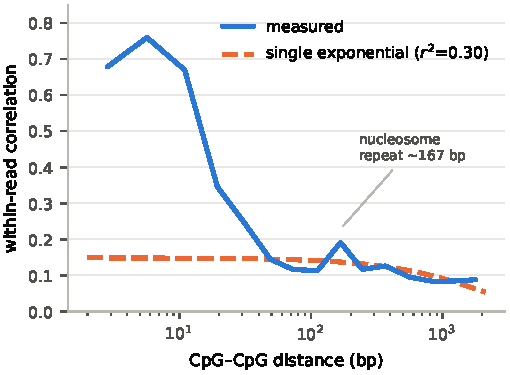
\includegraphics[width=0.62\textwidth]{figures/decay_curve.pdf}
\caption{Within-read methylation correlation against CpG--CpG distance,
HG00146 chr15 ($2{,}323$ windows of $2$\,kb, $\sim\!2.5$\,Mb, call-error
corrected). The single-exponential model assumed by
\texttt{simulate\_patterns.molecules\_markov} and by
\texttt{decay.comethylation\_decay}'s fit does not describe the data
($r^2 = 0.30$, against $>0.95$ on simulation).}
\label{fig:decay}
\end{figure}

Figure~\ref{fig:decay} is the first measurement of this quantity on the project's
data, and it refutes the model used to simulate it. The structure is
\textbf{two-component}: correlation peaks at $0.76$ around $6$\,bp, falls steeply
to $0.15$ by $49$\,bp --- a short-range decay length of order $20$--$25$\,bp ---
and then \emph{plateaus} at $0.07$--$0.09$ out to at least $1775$\,bp rather than
continuing to decay. A local bump at $167$\,bp coincides with the nucleosome
repeat length; on one donor and one bin that is suggestive, not a finding.

\subsection{The design effect, measured}

\begin{figure}[h]
\centering
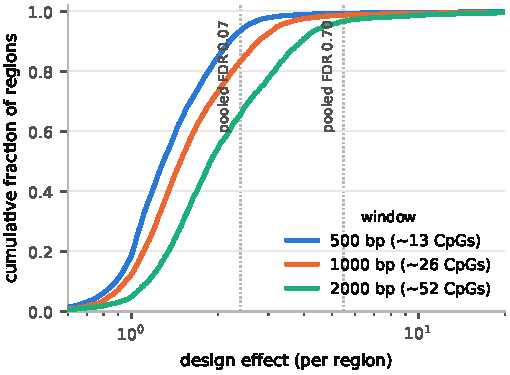
\includegraphics[width=0.62\textwidth]{figures/design_effect.pdf}
\caption{Distribution of the per-region design effect,
\texttt{readlevel.design\_effect} on HG00146 chr15, at three window sizes.
Dotted lines mark the design effects at which the pooled test's FDR was measured
in simulation. The caller's own regions are capped at $1000$\,bp.}
\label{fig:de}
\end{figure}

\begin{center}
\small
\begin{tabular}{lrrrrr}
\toprule
window & median DE & IQR & 90th pct & \% DE $>2$ & \% DE $>5$ \\
\midrule
\textbf{500\,bp} (the caller's scale) & \textbf{1.29} & 1.05--1.72 & 2.20 & 15\% & \textbf{0.7\%} \\
1000\,bp (\texttt{max\_span}) & 1.48 & 1.17--2.06 & 2.78 & 27\% & 1.5\% \\
2000\,bp & 1.89 & 1.43--2.84 & 3.91 & --- & 4.3\% \\
\bottomrule
\end{tabular}
\end{center}

Against the FDR-versus-DE curve of \S\ref{sec:bench}, this says:

\begin{quote}
\textbf{Region pooling is broadly defensible at the scale this caller actually
uses. The regime where it collapses is under $1\%$ of regions, not the typical
case.}
\end{quote}

This substantially demotes the read-level and pattern paths. The critique that
motivated them measured type I inflation at co-methylation $1.0$, i.e.\
$\mathrm{DE} = 5.5$, which is the \emph{99th percentile} of real regions rather
than the typical one. Paths B and C remain correct and worth having; the case for
making either the default is much weaker than it appeared. The defensible
architecture is \textbf{design-effect-aware}: pool where the measured DE is low,
fall back to the read-level path where it is not. Since DE is now measurable per
region, that is a switch, not a research programme.

\subsection{An unresolved disagreement}

\S\ref{sec:de} argued that having two independent estimators of the design effect
is a deliberate tripwire. It is currently tripped. At $2$\,kb they agree
(pooled long-range correlation $0.0733$ versus median per-window implied ICC
$0.0728$); at $500$\,bp they do not (\texttt{implied\_design\_effect} $2.77$
against a measured median of $1.29$). The likely cause is a summary mismatch ---
the correlation curve is pooled with variance weighting, so high-variance windows
dominate it, while the design effect is a median over windows, and at short range
the across-window spread is much larger. That is a hypothesis, not a
demonstration. \textbf{Until it is resolved, the direct per-region measurement is
the one to use}; it does not depend on the decay-curve machinery at all.

\section{Open problems}

\begin{enumerate}
\item \textbf{Resolve the design-effect estimator disagreement} (\S\ref{sec:real}).
The tripwire exists to be believed.
\item \textbf{Replace the single-exponential decay model} in both the fit and the
simulator with a two-component form (short exponential plus floor). The simulator
being misspecified against real correlation structure is the recurring failure
mode of this project.
\item \textbf{Switch errors are modelled in no test.} They move reads between
alleles, which attenuates $T_{\mathrm{MML}}$ and \emph{inflates}
$T_{\mathrm{NME}}$, since a mislabelled allele looks bistable. Two cohort donors
carry $\hat\rho$ five to ten times everyone else's with essentially zero
significant regions; that signature --- elevated $T_{\mathrm{NME}}$ with normal
$T_{\mathrm{MML}}$ --- would be close to a positive identification, and it is a
genome-wide aggregate, so it does not need the per-region power the entropy axis
lacks.
\item \textbf{The entropy axis may not be reachable.} Maximum power on equal-mean
disorder imbalance across every method and scenario tested was $0.034$;
$T_{\mathrm{NME}}$ scored $0.000$ on that axis in all three scenarios while
retaining power on the mean axis, i.e.\ at $10$--$30$ reads it largely tracks the
mean. The identifiability measurement explains why: at $400$ reads the MLE
recovers $(\alpha, \beta) = (1.2, 0.6)$ as $(1.26, 0.58)$; at $20$ reads it
returns $(1.81, 0.10)$.
\item \textbf{No haplotype-specific real-data validation yet.} Everything in
\S\ref{sec:real} is unphased, because co-methylation along a molecule is not a
haplotype quantity. Every ASM test remains blocked on haplotagged BAMs.
\end{enumerate}

\section*{Software}

\url{https://github.com/terencewtli/ont_asm_caller}. Paths A, B and C are
\texttt{model.py}/\texttt{region.py}, \texttt{readlevel.py}, and
\texttt{pattern.py}; nulls are \texttt{null.py}; correlation measurement is
\texttt{decay.py}; simulators are \texttt{simulate\_mixture.py},
\texttt{simulate\_reads.py} and \texttt{simulate\_patterns.py}. The figures here
are reproduced by \texttt{docs/paper/make\_figures.py}.

\end{document}
